\documentclass[11pt,a4paper]{article}

\usepackage[margin=2.2cm]{geometry}
\usepackage{amsmath,amssymb}
\usepackage{algorithm}
\usepackage{algpseudocode}
\usepackage{tikz}
\usetikzlibrary{arrows.meta,positioning,calc}
\usepackage{booktabs}
\usepackage{hyperref}

\title{LIF Action Mapping to Audio and MIDI Output}
\author{lif\_lova Technical Notes}
\date{\today}

\begin{document}
\maketitle

\section{Overview}

This document specifies how neural activity from a leaky integrate-and-fire (LIF) network
is converted to:
\begin{enumerate}
    \item tone synthesis output, and
    \item MIDI note output.
\end{enumerate}

The runtime pipeline has three logical stages:
\begin{itemize}
    \item \textbf{Input layer}: audio features (8-band spectrum and RMS) are mapped to neuron drive.
    \item \textbf{Hidden layer}: recurrent LIF neurons evolve according to topology-specific connectivity.
    \item \textbf{Output layer}: a sampled activity column is mapped to 16 bins, then to audio oscillators and MIDI notes.
\end{itemize}

\section{Neural Structure and Equations}

\subsection{Input Layer: Audio-to-Neuron Drive}

Let $b_g \in [0,1]$ be audio band energy for group $g \in \{0,\dots,7\}$ and $r \in [0,1]$ be RMS.
Each neuron $i$ is assigned a band index:
\begin{equation}
g(i) = \left\lfloor \frac{8i}{N} \right\rfloor
\end{equation}
where $N$ is neuron count.

With influence control $\alpha \in [0,1]$, define:
\begin{align}
\gamma(\alpha) &= 0.35 + 1.65\alpha, \\
u_i &= \gamma(\alpha)\left[b_{g(i)}\left(0.30 + 1.70r\right) + 0.15\,b_{(g(i)+3)\bmod 8}\right].
\end{align}

Here $u_i$ is the external input current to neuron $i$.

\subsection{Hidden Layer: LIF Dynamics}

Each neuron keeps membrane potential $v_i$, spike flag $s_i$, and refractory timer.
Using per-frame step $\Delta t$, parameters vary with influence:
\begin{align}
\lambda &= 0.70 - 0.45\alpha \quad \text{(leak)}, \\
\theta &= 0.75 - 0.35\alpha \quad \text{(threshold)}, \\
v_{\text{reset}} &= 0.04 + 0.10(1-\alpha), \\
\tau_{\text{ref}} &= 0.03 + 0.08(1-\alpha).
\end{align}

For weighted adjacency matrix $W = [w_{ji}]$:
\begin{equation}
I_i(t) = u_i(t) + \sum_{j=1}^{N} w_{ji}s_j(t).
\end{equation}

A discrete LIF update is modeled as:
\begin{equation}
v_i(t+\Delta t) =
\begin{cases}
v_{\text{reset}}, & \text{if refractory is active},\\
\operatorname{clip}\left((1-\lambda\Delta t)v_i(t) + \Delta t\,I_i(t),\,0,\,1\right), & \text{otherwise}.
\end{cases}
\end{equation}

Spike event:
\begin{equation}
s_i(t+\Delta t)=
\begin{cases}
1, & v_i(t+\Delta t) \ge \theta,\\
0, & \text{otherwise}.
\end{cases}
\end{equation}

On spike, $v_i \leftarrow v_{\text{reset}}$ and refractory timer is set to $\tau_{\text{ref}}$.

\subsection{Output Layer: Column Sampling to 16 Bins}

At scan phase $\phi \in [0,1]$, choose spatial column:
\begin{equation}
x = \operatorname{round}\left(\phi\,(G-1)\right)
\end{equation}
where $G$ is LIF grid size.

For output bin $k \in \{0,\dots,15\}$:
\begin{align}
y_k &= \operatorname{round}\left(\frac{k+0.5}{16}(G-1)\right),\\
e_k &= \operatorname{clip}\left(0.8\,v_{x,y_k} + 0.6\,s_{x,y_k},\,0,\,1\right).
\end{align}

The vector $\mathbf{e}=(e_0,\dots,e_{15})$ is the shared output for audio and MIDI mapping.

\section{Layered Signal-Flow Diagram}

\begin{center}
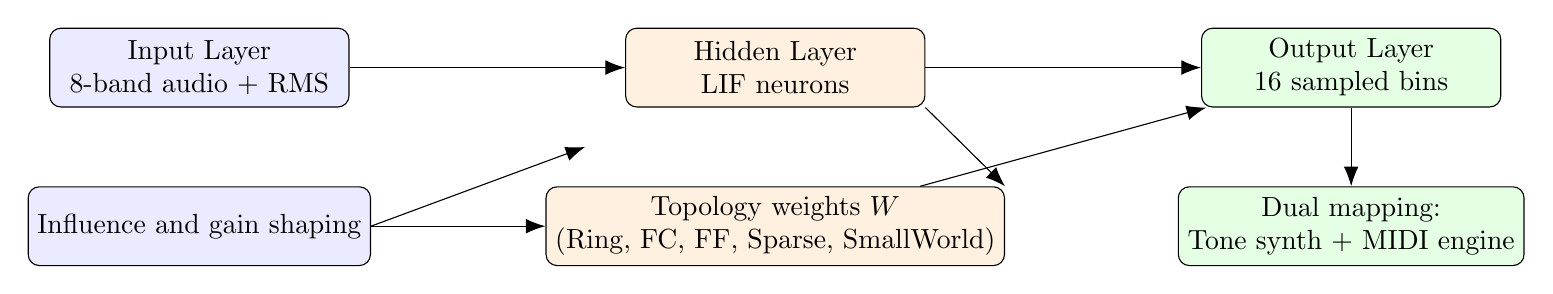
\begin{tikzpicture}[
    node distance=10mm and 10mm,
    box/.style={draw,rounded corners,minimum width=38mm,minimum height=10mm,align=center},
    arrow/.style={-{Latex[length=2.5mm]}}
]
    \node[box,fill=blue!8] (in1) {Input Layer\\8-band audio + RMS};
    \node[box,fill=blue!8,below=of in1] (in2) {Influence and gain shaping};

    \node[box,fill=orange!12,right=35mm of in1] (hid1) {Hidden Layer\\LIF neurons};
    \node[box,fill=orange!12,below=of hid1] (hid2) {Topology weights $W$\\(Ring, FC, FF, Sparse, SmallWorld)};

    \node[box,fill=green!10,right=35mm of hid1] (out1) {Output Layer\\16 sampled bins};
    \node[box,fill=green!10,below=of out1] (out2) {Dual mapping:\\Tone synth + MIDI engine};

    \draw[arrow] (in1) -- (hid1);
    \draw[arrow] (in2) -- (hid2);
    \draw[arrow] (hid1) -- (out1);
    \draw[arrow] (hid2) -- (out1);
    \draw[arrow] (in2.east) -- ($(hid1.west)!0.5!(hid2.west)$);
    \draw[arrow] (hid1.south east) -- (hid2.north east);
    \draw[arrow] (out1) -- (out2);
\end{tikzpicture}
\end{center}

\section{Topology Diagrams (Hidden Layer Connectivity)}

\subsection{Ring Topology}
\begin{center}
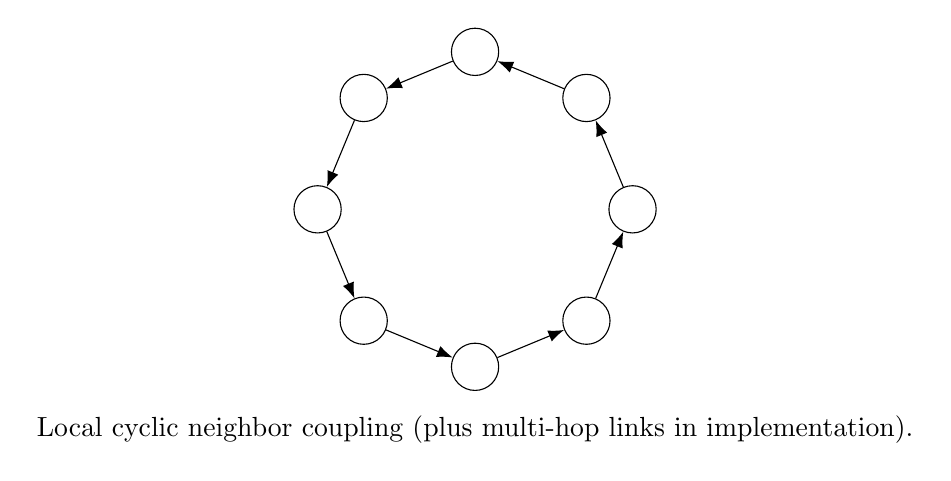
\begin{tikzpicture}[node/.style={circle,draw,minimum size=6mm},arrow/.style={-{Latex[length=2mm]}}]
    \foreach \i in {0,...,7} {
        \node[node] (n\i) at ({45*\i}:2.0) {};
    }
    \foreach \i/\j in {0/1,1/2,2/3,3/4,4/5,5/6,6/7,7/0} {
        \draw[arrow] (n\i) -- (n\j);
    }
    \node at (0,-2.8) {Local cyclic neighbor coupling (plus multi-hop links in implementation).};
\end{tikzpicture}
\end{center}

\subsection{Fully Connected Topology}
\begin{center}
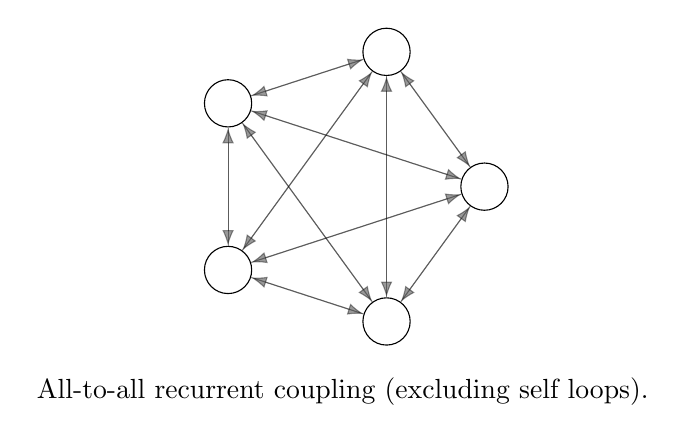
\begin{tikzpicture}[node/.style={circle,draw,minimum size=6mm},arrow/.style={-{Latex[length=2mm]}}]
    \foreach \i in {0,...,4} {
        \node[node] (n\i) at ({72*\i}:1.8) {};
    }
    \foreach \i in {0,...,4} {
        \foreach \j in {0,...,4} {
            \ifnum\i=\j\else
                \draw[arrow,opacity=0.4] (n\i) -- (n\j);
            \fi
        }
    }
    \node at (0,-2.6) {All-to-all recurrent coupling (excluding self loops).};
\end{tikzpicture}
\end{center}

\subsection{Feedforward Topology (Layer-Separated)}
\begin{center}
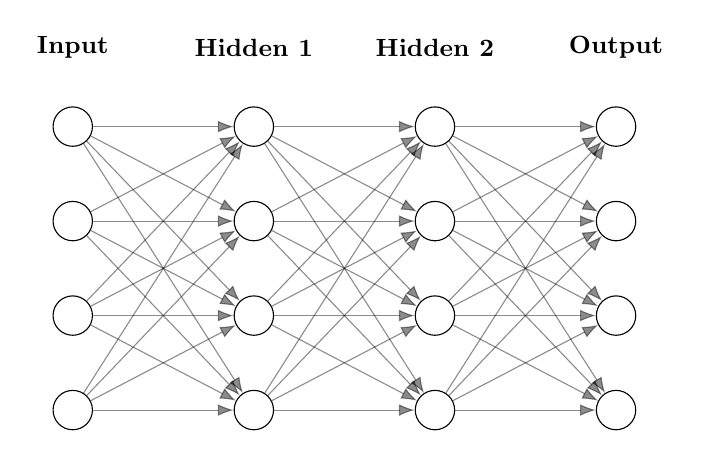
\begin{tikzpicture}[
    node/.style={circle,draw,minimum size=5mm},
    lbl/.style={font=\small\bfseries},
    arrow/.style={-{Latex[length=2mm]}}
]
    % Input layer
    \foreach \i in {0,...,3} { \node[node] (i\i) at (0, {1.8-\i*1.2}) {}; }
    \node[lbl] at (0,2.8) {Input};

    % Hidden layer 1
    \foreach \i in {0,...,3} { \node[node] (hA\i) at (2.3, {1.8-\i*1.2}) {}; }
    \node[lbl] at (2.3,2.8) {Hidden 1};

    % Hidden layer 2
    \foreach \i in {0,...,3} { \node[node] (hB\i) at (4.6, {1.8-\i*1.2}) {}; }
    \node[lbl] at (4.6,2.8) {Hidden 2};

    % Output layer
    \foreach \i in {0,...,3} { \node[node] (o\i) at (6.9, {1.8-\i*1.2}) {}; }
    \node[lbl] at (6.9,2.8) {Output};

    % Connections between consecutive layers only
    \foreach \a in {0,...,3} {
        \foreach \b in {0,...,3} {
            \draw[arrow,opacity=0.45] (i\a) -- (hA\b);
            \draw[arrow,opacity=0.45] (hA\a) -- (hB\b);
            \draw[arrow,opacity=0.45] (hB\a) -- (o\b);
        }
    }
\end{tikzpicture}
\end{center}

\subsection{Sparse Random and Small-World Topologies}
\begin{center}
\begin{tabular}{@{}ll@{}}
\toprule
Topology & Connectivity idea \\
\midrule
Sparse Random & Each directed edge exists with low probability (about 10\%). \\
Small-World & Mostly local ring-like edges plus occasional rewired shortcuts. \\
\bottomrule
\end{tabular}
\end{center}

\section{Algorithm Pseudocode}

\begin{algorithm}[H]
\caption{Input Layer: Audio Features to Neuron Drive}
\begin{algorithmic}[1]
\Require Bands $b[0..7]$, RMS $r$, influence $\alpha$, neuron count $N$
\For{$i=0$ to $N-1$}
    \State $g \gets \lfloor 8i/N \rfloor$
    \State $\text{bandDrive} \gets b[g] \cdot (0.30 + 1.70r)$
    \State $\text{cross} \gets 0.15 \cdot b[(g+3) \bmod 8]$
    \State $\gamma \gets 0.35 + 1.65\alpha$
    \State $u[i] \gets (\text{bandDrive} + \text{cross})\cdot \gamma$
\EndFor
\end{algorithmic}
\end{algorithm}

\begin{algorithm}[H]
\caption{Hidden Layer: LIF Network Step}
\begin{algorithmic}[1]
\Require Previous state $(v,s,\text{ref})$, input $u$, weights $W$, parameters $(\lambda,\theta,v_{reset},\tau_{ref})$
\For{$i=0$ to $N-1$}
    \State $I \gets u[i] + \sum_j W[j,i]\cdot s[j]$
    \If{$\text{ref}[i] > 0$}
        \State $\text{ref}[i] \gets \text{ref}[i] - \Delta t$
        \State $v[i] \gets v_{reset}$
        \State $s[i] \gets 0$
    \Else
        \State $v[i] \gets \operatorname{clip}((1-\lambda\Delta t)v[i] + \Delta t\,I, 0, 1)$
        \If{$v[i] \ge \theta$}
            \State $s[i] \gets 1$
            \State $v[i] \gets v_{reset}$
            \State $\text{ref}[i] \gets \tau_{ref}$
        \Else
            \State $s[i] \gets 0$
        \EndIf
    \EndIf
\EndFor
\end{algorithmic}
\end{algorithm}

\begin{algorithm}[H]
\caption{Output Layer: Column Sampling to 16 Energy Bins}
\begin{algorithmic}[1]
\Require LIF grid state $(v,s)$, scan phase $\phi \in [0,1]$
\State $x \gets \operatorname{round}(\phi\,(G-1))$
\For{$k=0$ to $15$}
    \State $y \gets \operatorname{round}(((k+0.5)/16)\cdot(G-1))$
    \State $e[k] \gets \operatorname{clip}(0.8\cdot v[x,y] + 0.6\cdot s[x,y], 0, 1)$
\EndFor
\State \Return $e[0..15]$
\end{algorithmic}
\end{algorithm}

\begin{algorithm}[H]
\caption{Audio Mapping: Bins to Additive Oscillator Bank}
\begin{algorithmic}[1]
\Require Energies $e[0..15]$, min/max frequency $(f_{min}, f_{max})$, sample rate $F_s$
\For{$k=0$ to $15$}
    \State $t \gets k/15$
    \State $f[k] \gets f_{min}\cdot (f_{max}/f_{min})^{t}$ \Comment{log-frequency spacing}
\EndFor
\For{each audio frame}
    \State $x \gets 0$
    \For{$k=0$ to $15$}
        \State $a[k] \gets a[k] + 0.01\cdot(e[k]-a[k])$ \Comment{amplitude smoothing}
        \State $\varphi[k] \gets \varphi[k] + 2\pi f[k]/F_s$
        \State $x \gets x + \sin(\varphi[k])\cdot a[k]$
    \EndFor
    \State output sample $\gets \operatorname{clip}(0.5x/16,-1,1)$
\EndFor
\end{algorithmic}
\end{algorithm}

\begin{algorithm}[H]
\caption{MIDI Mapping: Bins to Notes and Velocity}
\begin{algorithmic}[1]
\Require Energies $e[0..15]$, style, modal scale, key, note range
\State $e_{max} \gets \max_k e[k]$
\State $\tau_{on} \gets \max(0.18, 0.55\,e_{max})$
\State $\tau_{off} \gets \max(0.12, 0.40\,e_{max})$
\For{$k=0$ to $15$}
    \State compute harmonic function $F_k \in \{T,S,D\}$ from bin index and local contour
    \State choose chord notes from $(F_k, \text{style}, \text{modal scale}, \text{key})$
    \State map notes into configured MIDI range
    \If{feedforward topology}
        \State use pulse gate + cooldown scheduling
        \State velocity $\gets \operatorname{clip}(30 + 97\,e[k]^{0.7} + 10\,e[k-1], 30,127)$
    \Else
        \If{note is OFF and $e[k] > \tau_{on}$}
            \State velocity $\gets \operatorname{clip}(20 + 107\,(e[k]/\max(e_{max},\epsilon))^{0.65},20,127)$
            \State send NoteOn for chord notes
        \ElsIf{note is ON and $e[k] \le \tau_{off}$}
            \State send NoteOff for active notes
        \EndIf
    \EndIf
\EndFor
\end{algorithmic}
\end{algorithm}

\section{Audio and MIDI Output Mapping Summary}

\begin{center}
\begin{tabular}{@{}lll@{}}
\toprule
Signal & Audio output & MIDI output \\
\midrule
Bin index $k$ & Oscillator index/frequency channel & Harmonic role and register \\
Bin energy $e_k$ & Oscillator amplitude & Gate and velocity \\
Scan phase $\phi$ & Time-varying timbre source & Time-varying note activity \\
Topology & Activity texture and transients & Sustained vs pulsed articulation \\
\bottomrule
\end{tabular}
\end{center}

\section{Notes on Layer Differentiation}

\begin{itemize}
    \item \textbf{Input layer} contains externally observed features only (audio bands, RMS, influence controls).
    \item \textbf{Hidden layer} contains recurrent neural state and topology-defined coupling.
    \item \textbf{Output layer} is the 16-bin activity vector, consumed by both audio synthesis and MIDI generation.
\end{itemize}

\end{document}